\documentclass[xcolor={dvipsnames}]{beamer}
\usepackage[utf8]{inputenc}
\usetheme{Rochester}
\beamertemplatenavigationsymbolsempty
\setbeamercolor*{structure}{bg=Mahogany!20,fg=Mahogany}

\setbeamercolor*{palette primary}{use=structure,fg=white,bg=structure.fg}
\setbeamercolor*{palette secondary}{use=structure,fg=white,bg=structure.fg!75}
\setbeamercolor*{palette tertiary}{use=structure,fg=white,bg=structure.fg!50!black}
\setbeamercolor*{palette quaternary}{fg=white,bg=black}

\setbeamercolor{section in toc}{fg=black,bg=white}
\setbeamercolor{alerted text}{use=structure,fg=structure.fg!50!black!80!black}

\setbeamercolor{titlelike}{parent=palette primary,fg=structure.fg!50!black}
\setbeamercolor{frametitle}{bg=Mahogany,fg=white}

\setbeamercolor*{titlelike}{parent=section in toc}
% \usecolortheme{beaver}

%% Paquetes adicionales
\usepackage{multicol}
\usepackage{ragged2e}
\usepackage{tikz}

\title[Docker for dummies] {Docker for dummies}
\author[Leandro Kollenberger]
{Leandro Kollenberger}
\institute[redbee] {
redbee studios
}
\date[dockerpres] {
  30 de Marzo de 2018
}
\subject {Docker for dummies}
\titlegraphic{\vspace{-2cm}}
% \titlegraphic{
\includegraphics[height=.5\textheight]{assets/docker_logo.png}}

\pgfdeclareimage[height=0.5cm]{left-logo}{assets/redbee_logo.png}

\setbeamertemplate{sidebar left}
{
\logo{\pgfuseimage{left-logo}}
\vfill%
\rlap{\hskip0.1cm\insertlogo}%
%\vskip15pt%
\vskip5pt%
}

\begin{document}

\begin{frame}
   \tikz [remember picture,overlay]
    \node at
        % ([yshift=3cm]current page.south) 
        ([yshift=1.8cm]current page.center)
        {
\includegraphics[height=.5\textheight]{assets/docker_logo.png}};
   \titlepage
\end{frame}

% \frame{\titlepage}

\begin{frame}
  \frametitle{¿Qué es Docker?}
  \vspace{-0.8cm}
  \begin{multicols}{2}
  %\raggedright
  \justify
  Son tecnologías de memoria estática (SRAM), cuya velocidad se ajusta al
  ciclo de reloj del procesador, a diferencia de la DRAM.
  Desde el punto de vista funcional, la caché se utiliza como memoria
  intermedia entre el procesador y la DRAM, almacenando en forma temporal la
  información con la que se accede con más frecuencia en esta última.
  \columnbreak
  \vspace*{\fill}
  \vspace*{\fill}
  \end{multicols}
\end{frame}

%% Fin de la presentación!
\begin{frame}
  \vspace{-0.8cm}
  \begin{center}
    %% Foto de Perón
    \begin{figure}
    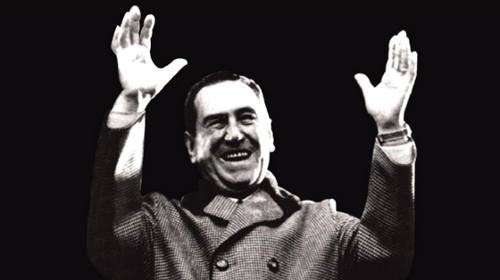
\includegraphics[width = 0.8\textwidth]{./assets/peron1.jpg}
    \end{figure}
    \Large{\textbf{Gracias! \\ Preguntas?}}
  \end{center}
\end{frame}

\end{document}
